The main program is composed of three main parts. The 2D correspondence extractor, the 3D reconstruction and pose estimation pipeline and the visualization module, for more information about each module, see their respective sections.



\begin{figure}[htb]
	\centering
	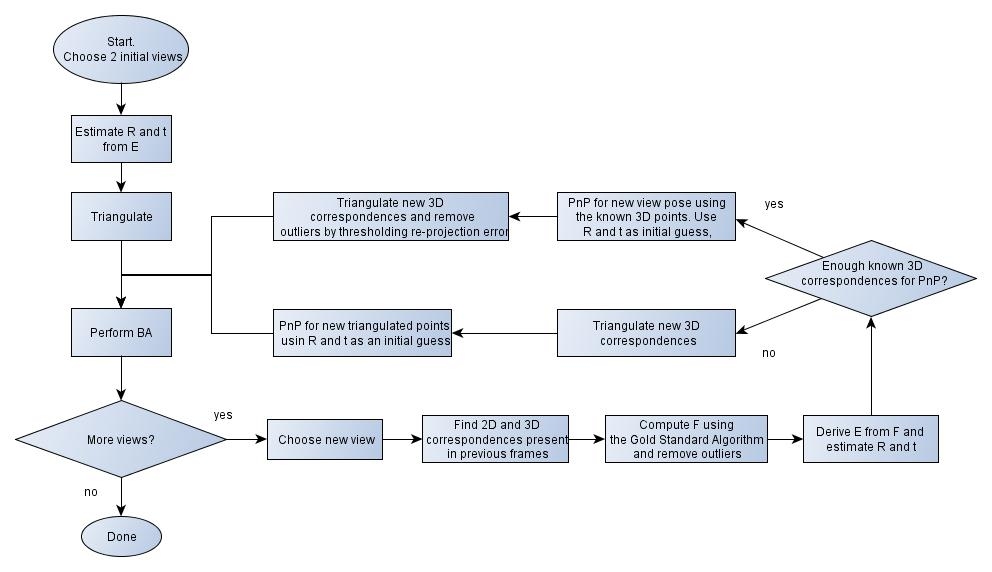
\includegraphics[width=160mm]{images/pipeline.jpg}
	\caption{\textit{Data flow between modules.}}
	\label{fig:block_overview_fig}  %Skapar referens till figuren
\end{figure}



\subsubsection{3D reconstruction pipeline}
The 3D reconstruction pipeline is where the image point pairs are used to triangulate 3D point estimates and estimate the camera poses (rotation and translation) relative to the first camera. A rough flowchart of the main program is included below.

Data from the reconstruction is saved in the propietary .alx format after adding a new camera, and after bundle adjustment for this camera.